\setproblem
    {B}
    {주차장 정산 시스템}

\section{\pid. \pname}

\begin{frame} % No title at first slide
    \sectiontitle{\pid}{\pname}
    \sectionmeta{
        출제자:박준형(\idtext{refill447})\\
        태그: \tagtext{\#set, \#hash\_set, \#tree\_set}\\
        예상 난이도: \tiertext{Silver5}
    }
    \begin{itemize}
        \item 제출 33번, 정답 18명 (정답률 54.5\%)
        \item 처음 푼 사람: 김0건 9분
    \end{itemize}
\end{frame}
%----------------------------------------------------------------------------
\begin{frame}{\textbf{\pid}. \pname}
    \begin{itemize}
        \item 핵심은 각 차량의 입차/출차 시간의 차이를 계산하는 것입니다.
        \begin{enumerate}
            \item 차량별로 입차 시간을 저장한다. 
            \item 출차 기록을 만나면 주차 시간을 계산한다.
            \item 계산된 주차 시간을 저장한다.
            \item 모든 기록 처리가 끝나면 각 차량의 요금을 계산한다.
            \item 차량 번호 기준으로 정렬 후 출력한다.
        \end{enumerate}
    \end{itemize}
\end{frame}
%----------------------------------------------------------------------------
\begin{frame}{\textbf{\pid}. \pname}
    \begin{columns}[T]

    % 왼쪽
    \begin{column}{0.35\textwidth}
        \begin{itemize}
            \item 구현(파이썬 코드)
        \end{itemize}

        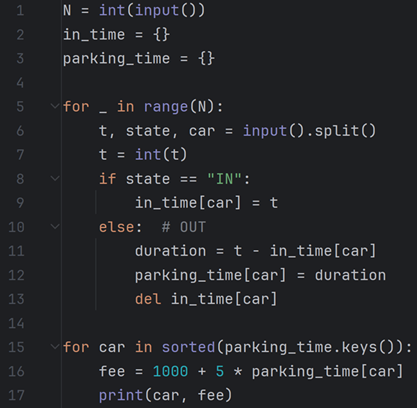
\includegraphics[width=\linewidth]{images/solution-code.png}
    \end{column}

    % 오른쪽
    \begin{column}{0.55\textwidth}
        \begin{itemize}
            \item 시간 복잡도
        \end{itemize}

        해시맵 사용 시,\\
        기록 처리: $O(1)\cdot O(N)=O(N)$\\
        정렬: $O(M \log M) (M = \text{차량 수}=N/2)$\\
        결과: $O(N \log N)$

        \bigskip

        트리맵 사용 시,\\
        기록 처리: $O(\log N) \cdot O(N) = O(N \log N)$\\
        결과: $O(N \log N)$
    \end{column}

\end{columns}
\end{frame}
%----------------------------------------------------------------------------
\begin{frame}{\textbf{\pid}. \pname}
    \begin{itemize}
        \item 별해\\
        $N \le 1\,000$이므로,\\
        IN에 대해 모든 $\texttt{\{car\_number,in\_time\}}$ 쌍을 배열에 담고,\\
        OUT에 대해 브루트포스로 차량 번호를 찾아\\
        $\texttt{in\_time}$과 비교하여 계산할 수 있습니다.\\
        따라서 비용을 계산하는 데 $O(N^2)$의 비용이 듭니다.\\
        마찬가지로 $O(N^2)$ 정렬을 사용할 수 있습니다.
        
    \end{itemize}
\end{frame}